%% 
%%  An UIT Edition example
%% 
%%  Example 04-27-26 on page 146.
%% 
%%  Copyright (C) 2012 Vo\ss 
%% 
%%  It may be distributed and/or modified under the conditions
%%  of the LaTeX Project Public License, either version 1.3
%%  of this license or (at your option) any later version.
%% 
%%  See http://www.latex-project.org/lppl.txt for details.
%% 

% Show page(s) 1,2,3

%% ==== 
\PassOptionsToClass{}{beamer}
\documentclass[aspectratio=169]{beamer}
\usepackage[utf8]{inputenc}

%\StartShownPreambleCommands
\usepackage{amsmath,esint}
\usepackage[british]{babel}
\usetheme{Warsaw}
\usecolortheme{rose}

%\usetheme{metropolis}
%\usepackage{appendixnumberbeamer}

%\StopShownPreambleCommands
\usepackage{pgfplots}
\usepackage{ mathrsfs }
\usepackage{caption}

\usepackage{gensymb}
\usepackage{color}
\usepackage{url}
\usetikzlibrary{shapes,backgrounds,calc}

\usepackage{tkz-euclide}
\usetkzobj{all}
\usepackage{tkz-fct}  
\usetikzlibrary{calc}
\usepackage{tikz,calc}

\usepackage[ruled]{algorithm2e}
\usepackage{tikz}
\usetikzlibrary{arrows.meta}
\usepackage{animate}
\DeclareMathOperator*{\minimize}{minimize}

\addtobeamertemplate{navigation symbols}{}{%
    \usebeamerfont{footline}%
    \usebeamercolor[fg]{footline}%
    \hspace{1em}%
    \insertframenumber/\inserttotalframenumber
}

\renewcommand{\thealgocf}{}

\begin{document}


\renewcommand{\thefootnote}{$\star$} 

\tikzset{
    o/.style={
        shorten >=#1,
        decoration={
            markings,
            mark={
                at position 1
                with {
                    \draw circle [radius=#1];
                }
            }
        },
        postaction=decorate
    },
    o/.default=2pt
}

\newcommand\derivative[5]{%
    \tkzDefPointByFct[draw](#1) \tkzGetPoint{start}
  \tkzDefPointByFct[draw](#2) \tkzGetPoint{end}
  \draw[thin,|-|,yshift=-3pt] (start) -- node[black,fill=white,#5] {#3}(start-|end);  
  \draw[thin,|-|,xshift=3pt] (start-|end) -- node[black,fill=white,right] {#4}(end); 
  %\draw[thin] (start) --(end); 
}

\title{Lecture 3}
\author{Mitesh M. Khapra}
\maketitle

\begin{frame}
\begin{align*}
\frac{\partial y}{\partial w_1} and \frac{\partial y}{\partial w_2}
\end{align*}
\end{frame}

\begin{frame}

\begin{table}[h!]
\begin{center}
\begin{tabular}{cccc}
 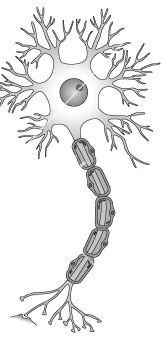
\includegraphics[scale=0.3]{images/InactiveNeuron.jpg}
 &            \begin{tikzpicture}
              \node[name=s,shape=circle split,draw=gray!40,line width=0mm,minimum size=1cm] {};  
            \begin{scope}[on background layer]
                \fill[black!50] (s.base) ([xshift=-0mm]s.east) arc (0:180:0.5cm-0mm)--cycle;
                \fill[white!50] (s.base) ([xshift=0mm]s.west) arc (180:360:0.5cm-0mm)--cycle;  
            \end{scope}
            \node (input0) at (-1.25, -1.25) {$x_1$};
            \node (input1) at (-0.75, -1.25) {$x_2$};
            \node (input2) at (0, -1.25) {$..$};
            \node (input3) at (0.75, -1.25) {$..$};
            \node (input4) at (1.25, -1.25) {$x_5$};
            \node (input5) at (0, -1.75) {$\in \{0,1\}$};

            \node (output) at (0, 1.25) {$y \in \{0,1\}$};

            %\node at (0,0.25) {$f$};
            \node at (0,-0.25) {$\theta$};

            \draw [->] (input0) -- (s.240);
            \draw [->] (input1) -- (s.255);
            \draw [->] (input2) -- (s.270);
            \draw [->] (input3) -- (s.285);
            \draw [->] (input4) -- (s.300);
            \draw [->] (s.90) -- (output);

            \end{tikzpicture}

&\tikzstyle{input_neuron}=[circle,draw=red!50,fill=orange!10,thick,minimum size=1mm]
\tikzstyle{hidden_neuron}=[circle,draw=blue!50,fill=blue!10,thick,minimum size=10mm]
\tikzstyle{output_neuron}=[circle,draw=green!50,fill=green!20,thick,minimum size=4mm]

\tikzstyle{input}=[circle,draw=black!50,fill=black!20,thick,minimum size=.2mm]

\begin{tikzpicture}
\node (input0) at (8,-0.1)  {$x_{1}$};
\node (input1) at (9,-0.1)  {$x_{2}$};
\node (input2) at (10,-0.1)  {$..$};
\node (input3) at (11,-0.1)  {$..$};
\node (input4) at (12,-0.1)  {$x_{n}$};

\node [hidden_neuron] (neuron1) at (10,2)  {};


\node (output0)  at (10,3.5) {$y$};

\draw [->] (input0) -- (neuron1);
\draw [->] (input1) -- (neuron1);
\draw [->] (input2) -- (neuron1);
\draw [->] (input3) -- (neuron1);
\draw [->] (input4) -- (neuron1);

\draw [->] (neuron1) -- (output0);

\node (formula)[scale=.8] at (8.1,0.6) {$w_{1}$};
\node (formula)[scale=.8] at (9.1,0.6) {$w_{2}$};
\node (formula)[scale=.8] at (9.8,0.6) {$..$};
\node (formula)[scale=.8] at (10.4,0.6) {$..$};
\node (formula)[scale=.8] at (11.1,0.6) {$w_{n}$};
\end{tikzpicture} 
&\begin{tikzpicture}[scale=0.75]

\draw[thick,->] (0,0) -- (3.5,0);
\draw[thick,->] (0,0) -- (0,3.5);

%\onslide<8->{\draw[densely dotted] (-1.2021,3.1111) -- (3.1111,-1.2021);}

\node at (3.3, -0.2) {$x_1$};
\node at (-0.2, 3.3) {$x_2$};

\node at (-0.1, -0.3) {$(0,0)$};
\node at (-0.1, 2.3) {$(0,1)$};
\node at (2.0, -0.3) {$(1,0)$};
\node at (2.2, 2.3) {$(1,1)$};
%\onslide<8->{\node at (-0.1, 1.0) {$-1 + 1.1x_1 + 1.1x_2 = 0$};}

\filldraw[blue] (0,0) circle (2pt);
\filldraw[red] (0,2) circle (2pt);
\filldraw[red] (2,0) circle (2pt);
\filldraw[blue] (2,2) circle (2pt);
\end{tikzpicture}\\

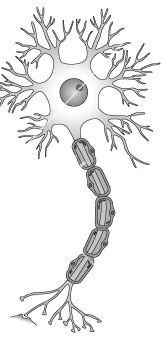
\includegraphics[scale=0.3]{images/InactiveNeuron.jpg}
 &            \begin{tikzpicture}
              \node[name=s,shape=circle split,draw=gray!40,line width=0mm,minimum size=1cm] {};  
            \begin{scope}[on background layer]
                \fill[black!50] (s.base) ([xshift=-0mm]s.east) arc (0:180:0.5cm-0mm)--cycle;
                \fill[white!50] (s.base) ([xshift=0mm]s.west) arc (180:360:0.5cm-0mm)--cycle;  
            \end{scope}
            \node (input0) at (-1.25, -1.25) {$x_1$};
            \node (input1) at (-0.75, -1.25) {$x_2$};
            \node (input2) at (0, -1.25) {$..$};
            \node (input3) at (0.75, -1.25) {$..$};
            \node (input4) at (1.25, -1.25) {$x_5$};
            \node (input5) at (0, -1.75) {$\in \{0,1\}$};

            \node (output) at (0, 1.25) {$y \in \{0,1\}$};

            %\node at (0,0.25) {$f$};
            \node at (0,-0.25) {$\theta$};

            \draw [->] (input0) -- (s.240);
            \draw [->] (input1) -- (s.255);
            \draw [->] (input2) -- (s.270);
            \draw [->] (input3) -- (s.285);
            \draw [->] (input4) -- (s.300);
            \draw [->] (s.90) -- (output);

            \end{tikzpicture}

&\tikzstyle{input_neuron}=[circle,draw=red!50,fill=orange!10,thick,minimum size=1mm]
\tikzstyle{hidden_neuron}=[circle,draw=blue!50,fill=blue!10,thick,minimum size=10mm]
\tikzstyle{output_neuron}=[circle,draw=green!50,fill=green!20,thick,minimum size=4mm]

\tikzstyle{input}=[circle,draw=black!50,fill=black!20,thick,minimum size=.2mm]

\begin{tikzpicture}
\node (input0) at (8,-0.1)  {$x_{1}$};
\node (input1) at (9,-0.1)  {$x_{2}$};
\node (input2) at (10,-0.1)  {$..$};
\node (input3) at (11,-0.1)  {$..$};
\node (input4) at (12,-0.1)  {$x_{n}$};

\node [hidden_neuron] (neuron1) at (10,2)  {};


\node (output0)  at (10,3.5) {$y$};

\draw [->] (input0) -- (neuron1);
\draw [->] (input1) -- (neuron1);
\draw [->] (input2) -- (neuron1);
\draw [->] (input3) -- (neuron1);
\draw [->] (input4) -- (neuron1);

\draw [->] (neuron1) -- (output0);

\node (formula)[scale=.8] at (8.1,0.6) {$w_{1}$};
\node (formula)[scale=.8] at (9.1,0.6) {$w_{2}$};
\node (formula)[scale=.8] at (9.8,0.6) {$..$};
\node (formula)[scale=.8] at (10.4,0.6) {$..$};
\node (formula)[scale=.8] at (11.1,0.6) {$w_{n}$};
\end{tikzpicture} 
&\begin{tikzpicture}[scale=0.75]

\draw[thick,->] (0,0) -- (3.5,0);
\draw[thick,->] (0,0) -- (0,3.5);

%\onslide<8->{\draw[densely dotted] (-1.2021,3.1111) -- (3.1111,-1.2021);}

\node at (3.3, -0.2) {$x_1$};
\node at (-0.2, 3.3) {$x_2$};

\node at (-0.1, -0.3) {$(0,0)$};
\node at (-0.1, 2.3) {$(0,1)$};
\node at (2.0, -0.3) {$(1,0)$};
\node at (2.2, 2.3) {$(1,1)$};
%\onslide<8->{\node at (-0.1, 1.0) {$-1 + 1.1x_1 + 1.1x_2 = 0$};}

\filldraw[blue] (0,0) circle (2pt);
\filldraw[red] (0,2) circle (2pt);
\filldraw[red] (2,0) circle (2pt);
\filldraw[blue] (2,2) circle (2pt);
\end{tikzpicture}\\
\end{tabular}
\end{center}
\end{table}

\end{frame}


\begin{frame}
    \begin{figure}[ht]
        \begin{minipage}[b]{0.23\linewidth}
           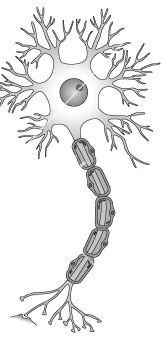
\includegraphics[width=0.5\textwidth]{images/InactiveNeuron.jpg}
        \end{minipage}
        %\hspace{0.1cm}
        \begin{minipage}[b]{0.23\linewidth}
            \begin{tikzpicture}
              \node[name=s,shape=circle split,draw=gray!40,line width=0mm,minimum size=1cm] {};  
            \begin{scope}[on background layer]
                \fill[black!50] (s.base) ([xshift=-0mm]s.east) arc (0:180:0.5cm-0mm)--cycle;
                \fill[white!50] (s.base) ([xshift=0mm]s.west) arc (180:360:0.5cm-0mm)--cycle;  
            \end{scope}
            \node (input0) at (-1.25, -1.25) {$x_1$};
            \node (input1) at (-0.75, -1.25) {$x_2$};
            \node (input2) at (0, -1.25) {$..$};
            \node (input3) at (0.75, -1.25) {$..$};
            \node (input4) at (1.25, -1.25) {$x_5$};
            \node (input5) at (0, -1.75) {$\in \{0,1\}$};

            \node (output) at (0, 1.25) {$y \in \{0,1\}$};

            %\node at (0,0.25) {$f$};
            \node at (0,-0.25) {$\theta$};

            \draw [->] (input0) -- (s.240);
            \draw [->] (input1) -- (s.255);
            \draw [->] (input2) -- (s.270);
            \draw [->] (input3) -- (s.285);
            \draw [->] (input4) -- (s.300);
            \draw [->] (s.90) -- (output);

            \end{tikzpicture}
        \end{minipage}
        %\hspace{0.1cm}
        \begin{minipage}[b]{0.22\linewidth}
            \tikzstyle{input_neuron}=[circle,draw=red!50,fill=orange!10,thick,minimum size=1mm]
            \tikzstyle{hidden_neuron}=[circle,draw=blue!50,fill=blue!10,thick,minimum size=10mm]
            \tikzstyle{output_neuron}=[circle,draw=green!50,fill=green!20,thick,minimum size=4mm]

            \tikzstyle{input}=[circle,draw=black!50,fill=black!20,thick,minimum size=.2mm]

            \begin{tikzpicture}[scale=0.75]
            \node (input0) at (8.5,-0.1)  {$x_{0}=1$};
            \node (input1) at (9.5,-0.1)  {$x_{1}$};
            \node (input2) at (10.5,-0.1)  {$..$};
            \node (input3) at (11.5,-0.1)  {$x_n$};
            %\node (input4) at (12,-0.1)  {$x_{n}$};
            %\node (input5) at (7,-0.1)  {$x_{0}=1$};

            \node [hidden_neuron] (neuron1) at (10,2)  {};


            \node (output0)  at (10,3.5) {$y$};

            \draw [->] (input0) -- (neuron1);
            \draw [->] (input1) -- (neuron1);
            \draw [->] (input2) -- (neuron1);
            \draw [->] (input3) -- (neuron1);
            %\draw [->] (input4) -- (neuron1);
            %\draw [->] (input5) -- (neuron1);

            \draw [->] (neuron1) -- (output0);

            \node (formula)[scale=.8] at (8.0,0.6) {$w_{0} = -\theta$};
            \node (formula)[scale=.8] at (9.3,0.6) {$w_{1}$};
            \node (formula)[scale=.8] at (10.1,0.6) {$..$};
            \node (formula)[scale=.8] at (10.8,0.6) {$w_{n}$};
            %\node (formula)[scale=.8] at (11.1,0.6) {$w_{n}$};
            %\node (formula)[scale=.8] at (7.2,0.6) {$w_{0} = -\theta$};

            \end{tikzpicture}

        \end{minipage}
        \begin{minipage}[b]{0.23\linewidth}
            \begin{tikzpicture}[scale=0.75]

            \draw[thick,->] (0,0) -- (3.5,0);
            \draw[thick,->] (0,0) -- (0,3.5);

            %\onslide<8->{\draw[densely dotted] (-1.2021,3.1111) -- (3.1111,-1.2021);}

            \node at (3.3, -0.2) {$x_1$};
            \node at (-0.2, 3.3) {$x_2$};

            \node at (-0.1, -0.3) {$(0,0)$};
            \node at (-0.1, 2.3) {$(0,1)$};
            \node at (2.0, -0.3) {$(1,0)$};
            \node at (2.2, 2.3) {$(1,1)$};
            %\onslide<8->{\node at (-0.1, 1.0) {$-1 + 1.1x_1 + 1.1x_2 = 0$};}

            \filldraw[blue] (0,0) circle (2pt);
            \filldraw[red] (0,2) circle (2pt);
            \filldraw[red] (2,0) circle (2pt);
            \filldraw[blue] (2,2) circle (2pt);
            \end{tikzpicture}
        \end{minipage}
        %\vspace{0.1cm}
        \begin{minipage}[b]{0.23\linewidth}
            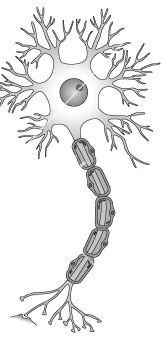
\includegraphics[width=0.56\textwidth]{images/InactiveNeuron.jpg}
        \end{minipage}
        %\hspace{0.1cm}
        \begin{minipage}[b]{0.23\linewidth}
            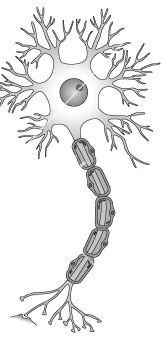
\includegraphics[width=0.4\textwidth]{images/InactiveNeuron.jpg}
        \end{minipage}
        \begin{minipage}[b]{0.23\linewidth}
            
            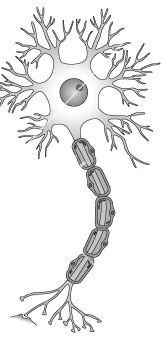
\includegraphics[width=0.5\textwidth]{images/InactiveNeuron.jpg}
        \end{minipage}
        %\hspace{0.1cm}
        \begin{minipage}[b]{0.23\linewidth}
            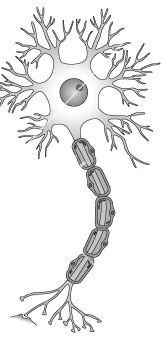
\includegraphics[width=0.4\textwidth]{images/InactiveNeuron.jpg}
        \end{minipage}
        %\vspace{0.1cm}
        
        \begin{minipage}[b]{0.23\linewidth}
            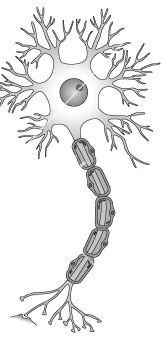
\includegraphics[width=0.35\textwidth]{images/InactiveNeuron.jpg}
        \end{minipage}
        %\hspace{0.1cm}
        \begin{minipage}[b]{0.23\linewidth}
            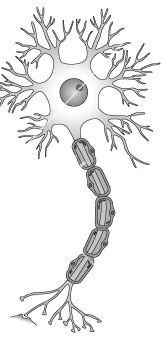
\includegraphics[width=0.4\textwidth]{images/InactiveNeuron.jpg}
        \end{minipage}
        %\hspace{0.1cm}
        \begin{minipage}[b]{0.23\linewidth}
            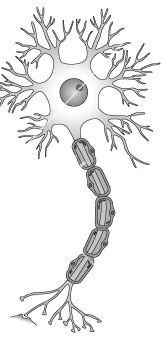
\includegraphics[width=0.4\textwidth]{images/InactiveNeuron.jpg}
        \end{minipage}
         \begin{minipage}[b]{0.23\linewidth}
          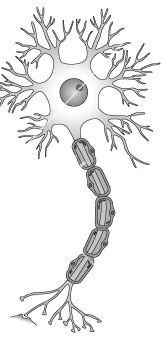
\includegraphics[width=0.4\textwidth]{images/InactiveNeuron.jpg}
         \end{minipage}
    \end{figure}
\end{frame}


\end{document}


